\documentclass[12pt,a4paper]{article}
\usepackage{geometry}
\usepackage{graphicx}
\usepackage{listings}
\usepackage{xcolor}
\usepackage{setspace}
\usepackage{array}
\usepackage{amsmath}

\geometry{margin=1in}
\singlespacing


\definecolor{codebg}{rgb}{0.95,0.95,0.95}
\lstset{
    backgroundcolor=\color{codebg},
    basicstyle=\ttfamily\footnotesize,
    frame=L,
    xleftmargin=15pt,
    framexleftmargin=10pt,
    numbers=left,
    numberstyle=\tiny\color{blue},
    breaklines=true,
    columns=flexible,
    escapeinside=``, % 允许转义到 LaTeX
    keywordstyle=\color{blue}\bfseries,
    commentstyle=\color{green!60!black},
    stringstyle=\color{purple},
    numberstyle=\tiny\color{gray},
    basicstyle=\ttfamily\small, % 稍大字体以便阅读
    showstringspaces=false,
    breaklines=true, % 允许自动换行
    breakatwhitespace=true, % 只在空格处换行
}


\title{CPT206 CW1 Week 6 Report - 2252377}
\date{05/04/2025} 

\begin{document}

\maketitle

\section{Code Explanation}
\subsection{Source code}
\begin{lstlisting}[language=Java]
public class Main {
    public static void main(String[] args) {
        System.out.println(countOccurrences("I have a banananana", "na"));//The result should be 4.
    }

    public static int countOccurrences(String input, String sub) {
        //First handle the boundary condition.
        if (sub == null || sub.isEmpty() || input.length() < sub.length()) {
            return 0;
        }
        
        //Using recursive techniques to count the times of repetition.
        int CountRepe = 0;
        if (input.startsWith(sub)) {
            CountRepe = 1;
        }
        return CountRepe + countOccurrences(input.substring(1), sub);
    }
}
\end{lstlisting}

\subsection{Key features:}
\begin{itemize}
\item Boundary condition: If the length of total input is less than that of the sub or null input, return 0.
\item Using recursion to count the total repetition times. Continuously extract the first character and compare it with the first character of the remaining string. Return 1 if they are the same, otherwise return 0. \\
Recursion sums up all these returned values to get the total number of repetitions.This method is quite similar to the 'factorial calculation'.\\ 
Visualization(example): 1+(1+(0+(1+(1+(0+(0+...
\item Initializing CountRepe to 0: recursive flow will add up values from all levels of recursion. If the condition is not met, adding 0 (the default value) will not affect the final result. This ensures the summation logic remains correct.
\end{itemize}

\section{Development \& Testing}
\subsection{Development Process}
\subsubsection{First programming}
I set the original boundary condition as: $input.length() < sub.length()$
\subsubsection{Improvement(assisted with Deepseek-R1)}
AI added two conditions to address cases where the substring is empty and deleted the 'equal' sign of my original condition.
To simplify the boundary conditions, I combined the three together.

\begin{figure}[h]
\centering
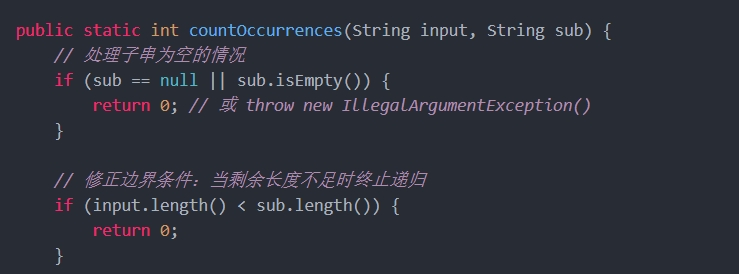
\includegraphics[width=0.7\textwidth]{CW1W6.png}
\caption{AI-assisted Code Improving}
\end{figure}


\subsection*{2.2 Testing}
\begin{tabular}{|l|m{2cm}|m{2cm}|m{2cm}|}
\hline
\textbf{input}&\textbf{sub}& \textbf{Expected} & \textbf{Actual} \\
\hline
"hello all!"  & "ll" & 2 & 2 \\
\hline
"an input string"  & "not a substring"& 0 & 0 \\
\hline
"I have a banananana"  & "na" &4& 4 \\
\hline 
"I have a pencil"  & "" &0& 0 \\
\hline 
"aaaaaaaaaa"&"aa"&9&9\\
\hline
\end{tabular}


\section*{3. Personal Reflection}

\begin{itemize}
\item The complexity of this method is O(n), which performs very well(each character checked only once). 
\item When using this method, there is a potential risk of integer overflow. However, for most string tests, the int type is generally sufficient. To ensure robustness and prevent overflow in extreme cases, it might be safer to replace int with long for the return type and counter variables.

\end{itemize}

\end{document}
